\chapter{Proposed Methods}
\lhead{Chapter 4. \emph{Proposed Methods}}
\label{chap.4}

This chapter presents the design, architecture, and implementation methodology of the Quantum Secure File Transfer Protocol (Q-SFTP). The system is built as a four-tier modular architecture integrating NIST-standardized post-quantum cryptographic (PQC) primitives with production-grade features including file integrity verification, resumable chunked transfers, role-based access control, metadata stripping, and a modern web interface.

\section{System Architecture}

Q-SFTP employs a four-tier, modularized architecture to protect confidentiality, integrity, and authentication of data in a post-quantum world. The four tiers are:

\begin{enumerate}
    \item \textbf{Client Layer (Web Browser):} A single-page web application using HTML5, CSS3, and vanilla JavaScript. Client-side BLAKE2b hashing is performed using the \texttt{blakejs} library. Transfer state persistence uses the browser's \texttt{localStorage} API, enabling resume across page reloads and session restarts.
    
    \item \textbf{Application Layer (Flask Web Server):} The Flask 3.x web server on port 5000 serves as the middleware between the browser and the PQC transport layer. It manages user authentication, transfer coordination, hash verification, privacy management, activity logging, and the admin panel.
    
    \item \textbf{Transport Layer (PQC Handshake Server):} The handshake server listens on TCP port 8888 and implements the four-phase Q-TLS handshake protocol using CRYSTALS-Kyber512 for key encapsulation and CRYSTALS-Dilithium2 for digital signatures. All file operations are routed through this encrypted channel.
    
    \item \textbf{Storage Layer (ServerStorage):} Server-side storage follows a directory-isolation model where each user has a private directory, plus a shared collaborative directory accessible to all authenticated users.
\end{enumerate}

Figure~\ref{fig:architecture} illustrates the overall structure of the Q-SFTP framework.

\begin{figure}[H]
    \centering
    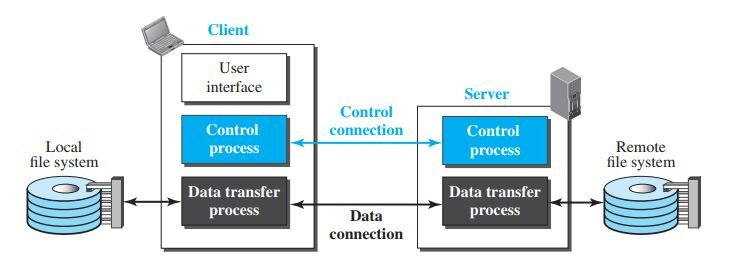
\includegraphics[width=0.85\textwidth]{Figures/FTP-architecture.png}
    \caption{Overall System Architecture of Q-SFTP}
    \label{fig:architecture}
\end{figure}

\section{Certificate Authority Design}

The Certificate Authority (CA) is a lightweight, self-contained module that issues and verifies post-quantum digital certificates using CRYSTALS-Dilithium. Unlike classical X.509 certificates that rely on RSA or ECDSA, the CA in Q-SFTP uses Dilithium2 for both signature generation and verification.

\begin{figure}[H]
    \centering
    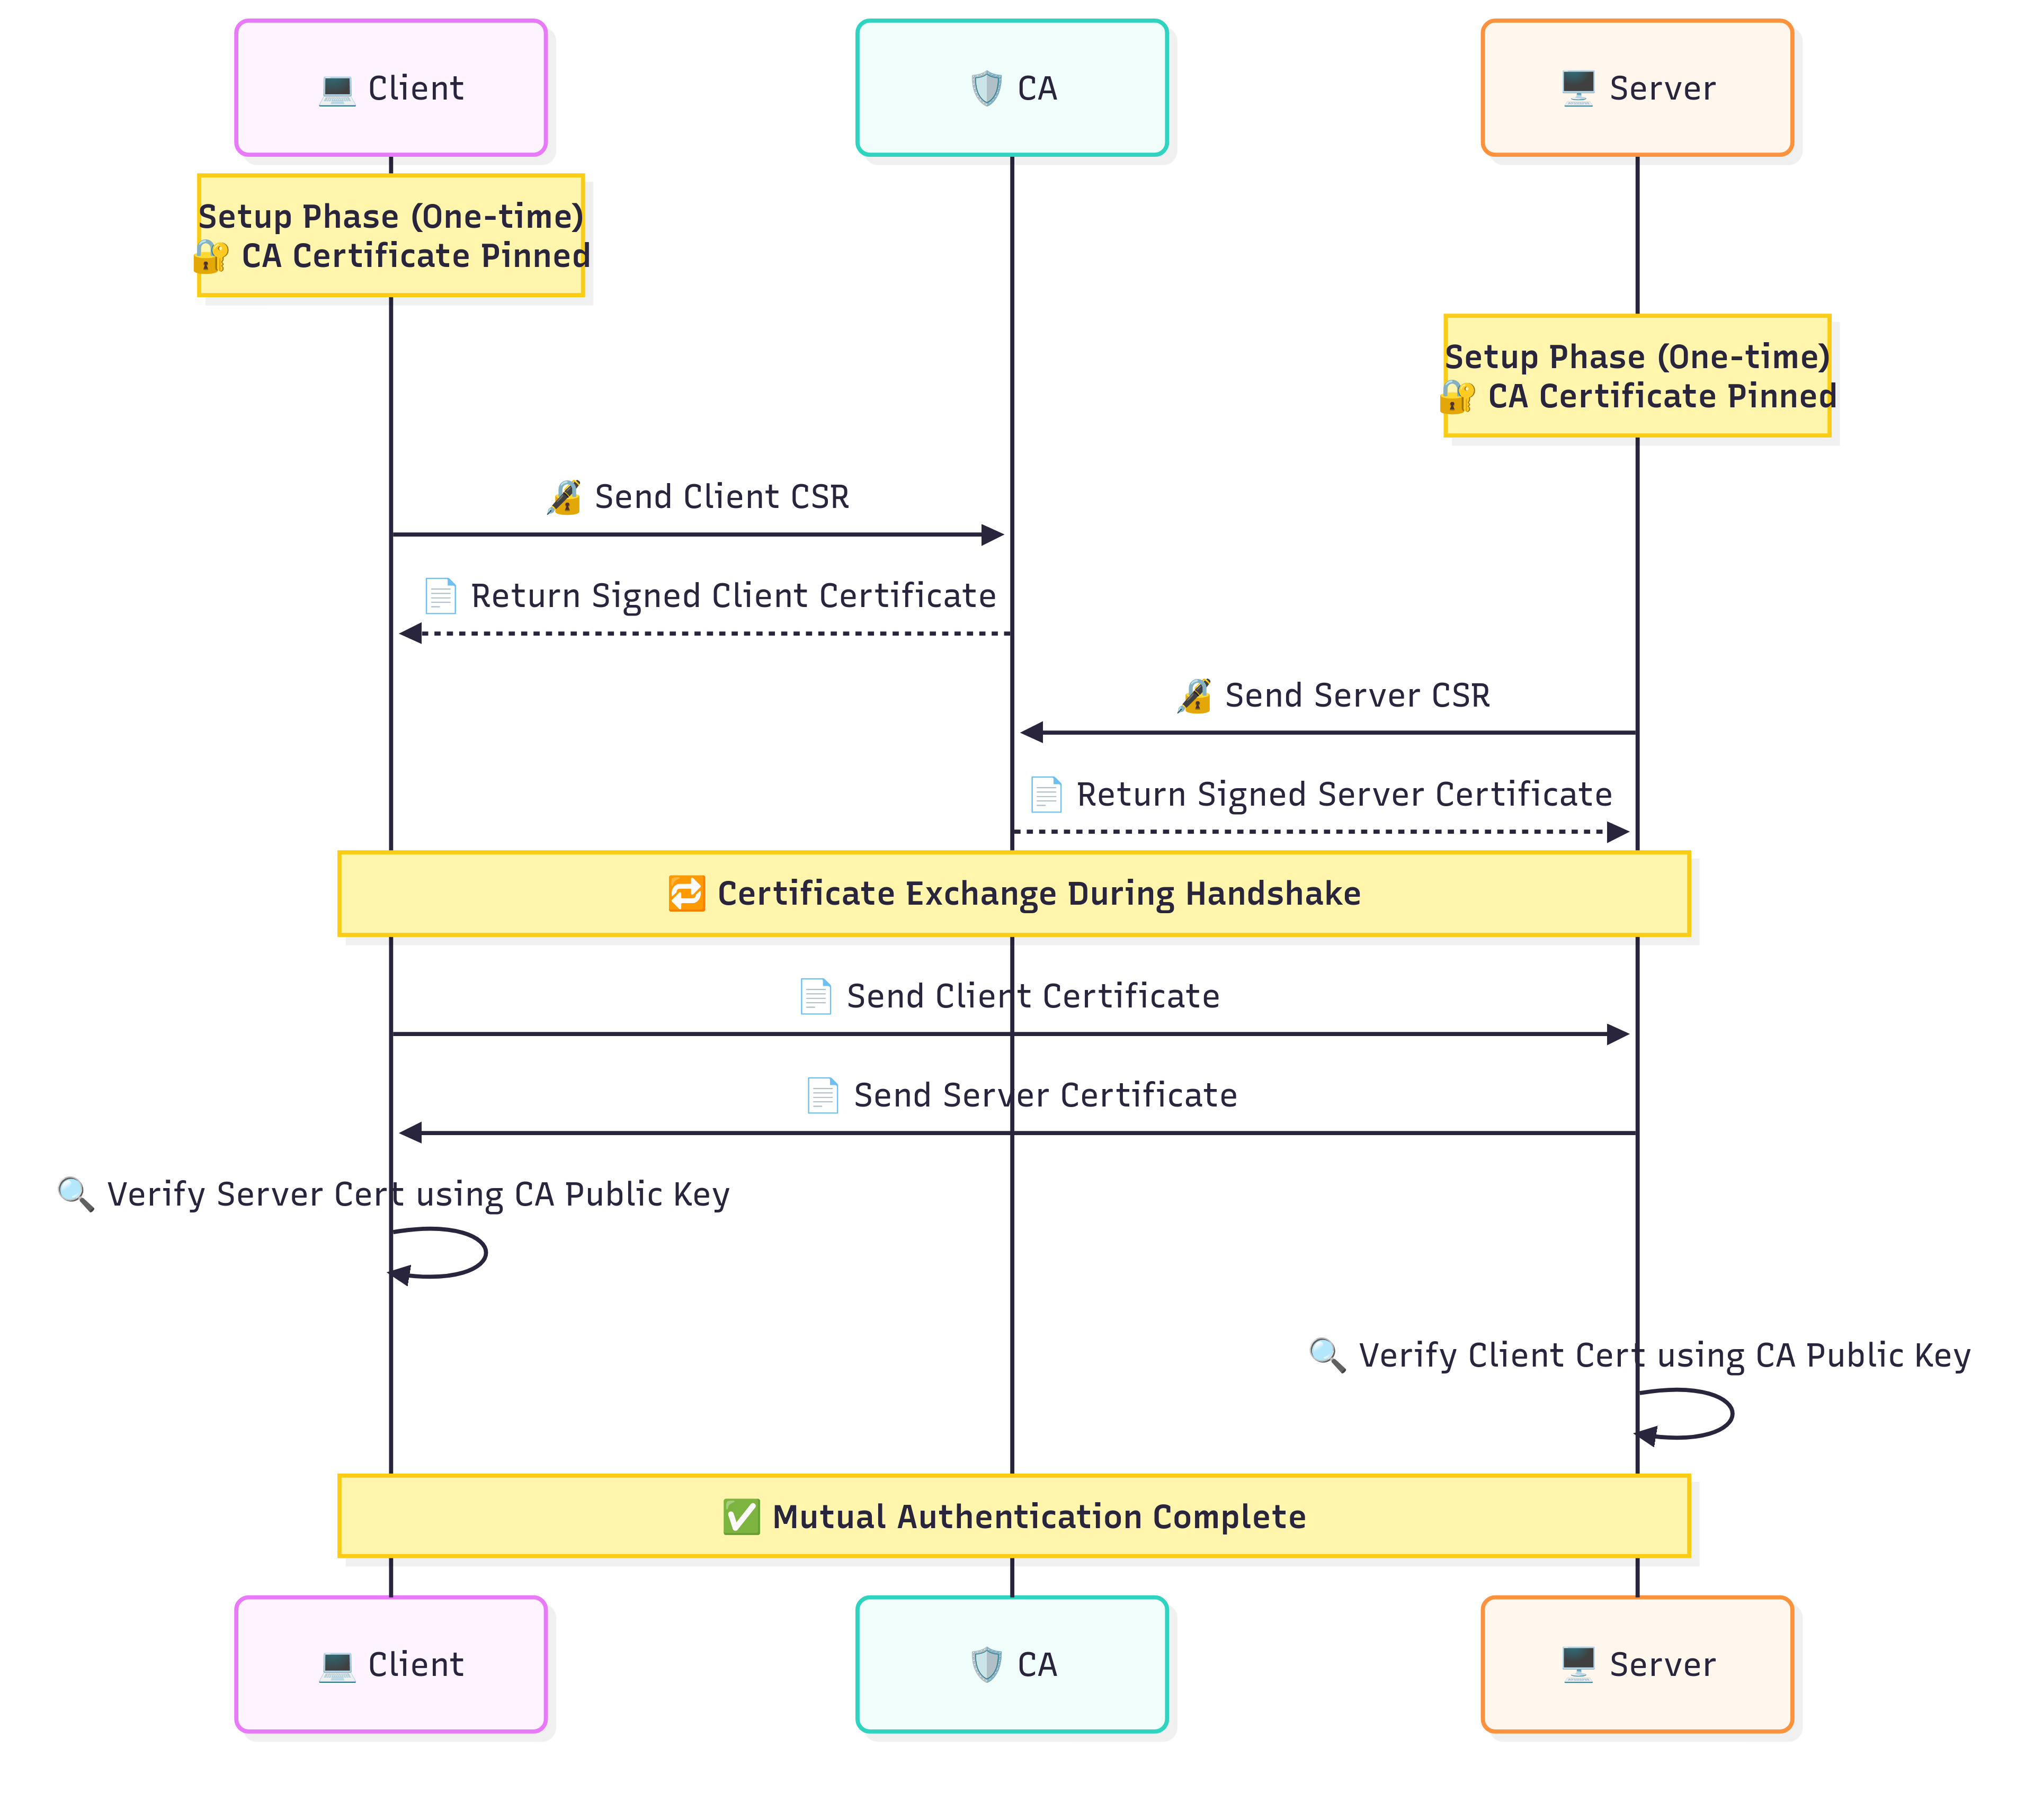
\includegraphics[width=0.8\textwidth]{Figures/CA.png}
    \caption{Architecture of the Quantum-Safe Certificate Authority}
    \label{fig:ca_architecture}
\end{figure}

\subsection{Certificate Format (Q-Cert)}

The custom certificate format retains common X.509 fields while adding support for post-quantum public keys and signatures:

\begin{itemize}
    \item \textbf{Subject:} Entity identifier (e.g., ``Server'', ``admin'', ``bob'')
    \item \textbf{Issuer:} CA identifier
    \item \textbf{Public\_Key:} Hex-encoded Dilithium2 public key (1,312 bytes)
    \item \textbf{Valid\_From / Valid\_Until:} ISO 8601 validity period
    \item \textbf{Signature:} Dilithium2 signature over all preceding fields
\end{itemize}

\begin{figure}[H]
    \centering
    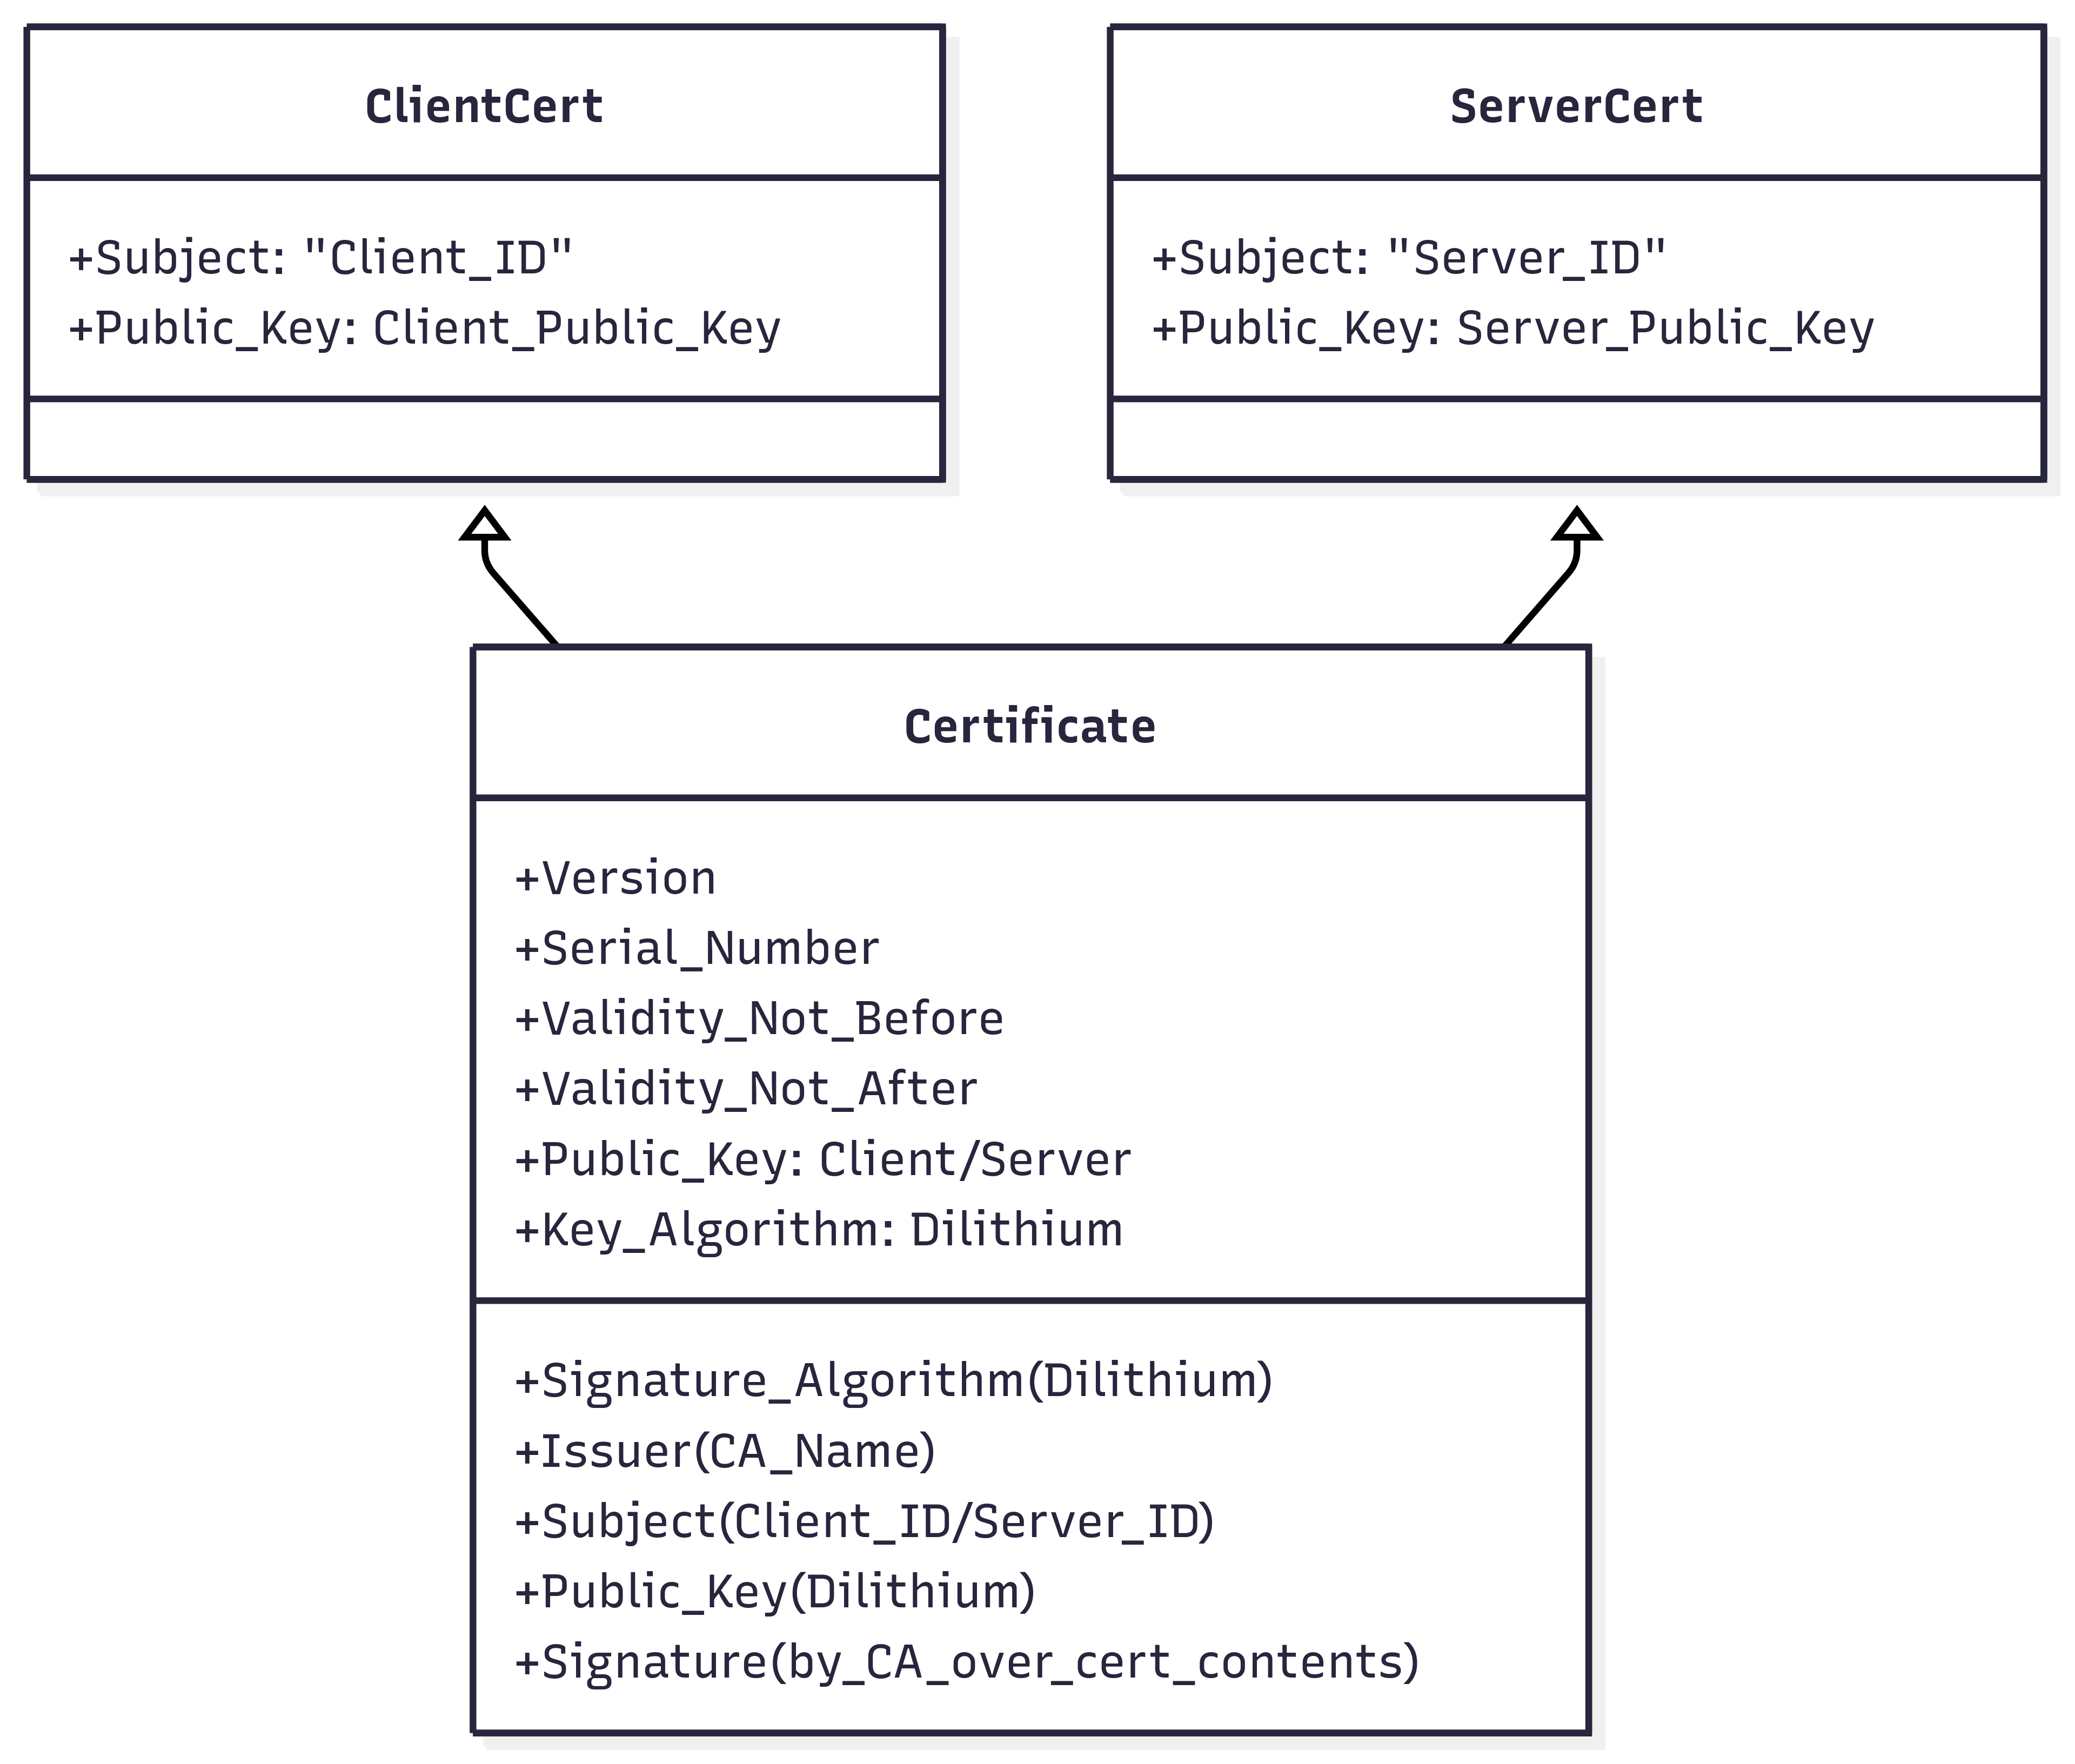
\includegraphics[width=0.75\textwidth]{Figures/Certificate.png}
    \caption{Structure of the Post-Quantum Digital Certificate (Q-Cert)}
    \label{fig:certificate_format}
\end{figure}

\section{Q-TLS Handshake Protocol}

The Q-TLS handshake replaces classical RSA/ECDHE-based key exchange with CRYSTALS-Kyber512 and uses Dilithium2 for mutual authentication. The protocol operates in four phases:

\subsection{Phase 1: Hello Exchange}

\begin{enumerate}
    \item The client generates a random nonce $N_C$ and a UTC timestamp $T_C$, then sends a \textit{ClientHello} message containing its digital certificate, nonce, and timestamp.
    \item The server verifies the client certificate against the CA's public key, checks that $|T_S - T_C| < 30$ seconds (replay protection), and generates a Kyber512 key pair $(pk_{Kyber}, sk_{Kyber})$.
    \item The server creates a Dilithium2 signature over the concatenation of $N_C$, its own nonce $N_S$, and $pk_{Kyber}$:
    \[
    \sigma_S = \text{Dilithium2.Sign}(sk_S^{Dil}, N_C \| N_S \| pk_{Kyber})
    \]
    \item The server responds with a \textit{ServerHello} containing its certificate, Kyber public key, nonce, and signature.
\end{enumerate}

\subsection{Phase 2: Key Encapsulation (Kyber512)}

\begin{enumerate}
    \item The client verifies $\sigma_S$, then encapsulates a shared secret using the server's Kyber public key:
    \[
    (ct, ss) = \text{Kyber512.Encaps}(pk_{Kyber})
    \]
    \item The client sends $ct$ (ciphertext, 768 bytes) to the server.
    \item The server decapsulates to recover the shared secret:
    \[
    ss = \text{Kyber512.Decaps}(sk_{Kyber}, ct)
    \]
\end{enumerate}

\subsection{Phase 3: Mutual Authentication and Key Derivation}

\begin{enumerate}
    \item The client computes a transcript hash over all exchanged messages:
    \[
    h_{transcript} = \text{SHA-256}(\text{ClientHello} \| \text{ServerHello} \| \text{ClientKeyShare})
    \]
    \item The client signs the transcript hash: $\sigma_C = \text{Dilithium2.Sign}(sk_C^{Dil}, h_{transcript})$
    \item The server verifies $\sigma_C$, confirming mutual authentication.
    \item Both parties derive the session key:
    \[
    K_{session} = \text{HKDF-SHA256}(ss, \text{salt} = \text{SHA-256}(N_C \| N_S), \text{info} = \text{``Q-SFTP-SESSION-KEY''})
    \]
\end{enumerate}

\subsection{Phase 4: Secure Data Transfer}

All subsequent communication is encrypted with AES-256-GCM using $K_{session}$, where each message uses a unique 96-bit nonce. The GCM authentication tag provides both confidentiality and integrity.

\begin{figure}[p]
    \centering
    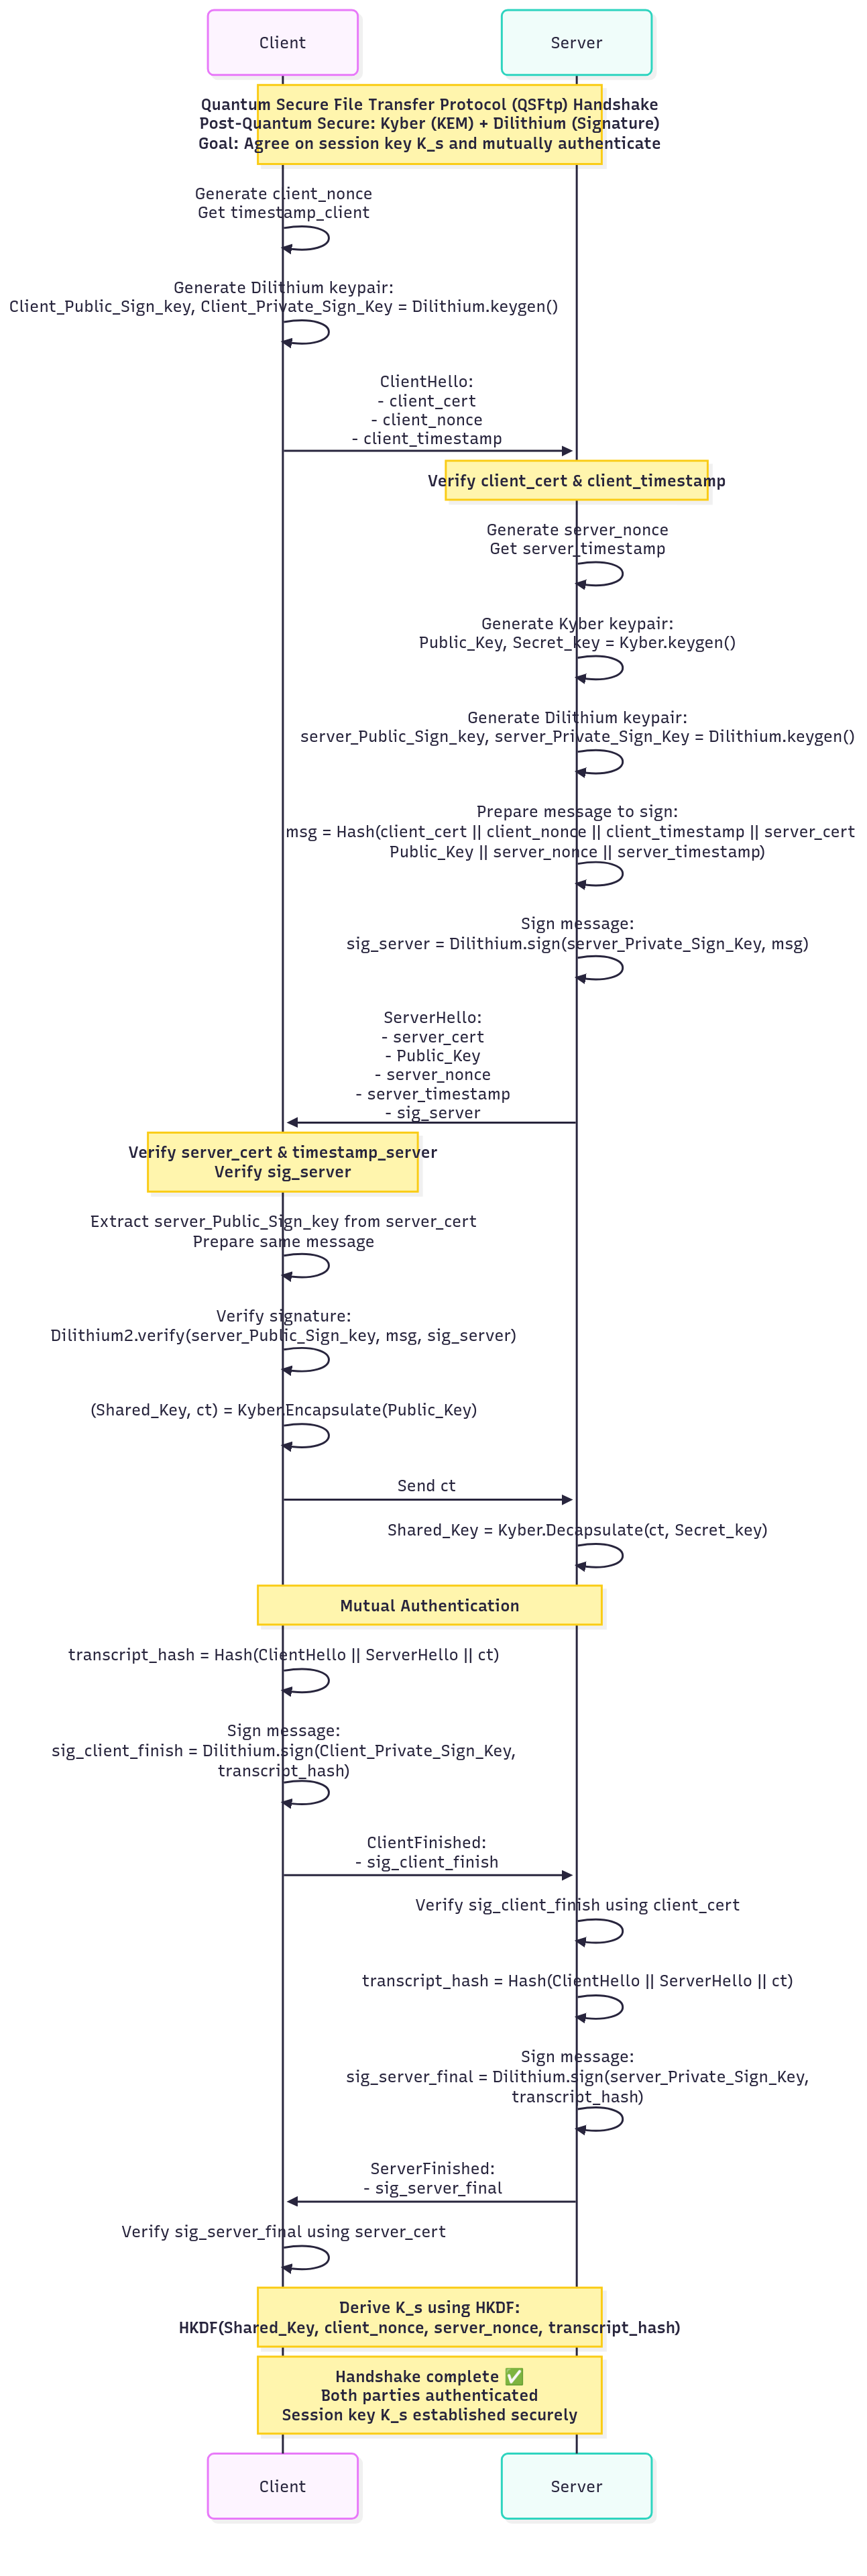
\includegraphics[height=\textheight]{Figures/Handshake.png}
    \caption{Proposed Quantum-TLS (Q-TLS) Handshake Sequence}
    \label{fig:handshake}
\end{figure}

\subsection{Handshake Algorithm}

Algorithm~\ref{algo:handshake} summarizes the Q-TLS handshake procedure.

\begin{algorithm}[H]
\caption{Q-TLS Handshake Protocol}
\label{algo:handshake}
\begin{algorithmic}[1]
\State Client generates $(N_C, T_C)$
\State Client $\rightarrow$ Server: \textit{ClientHello}(Cert$_C$, $N_C$, $T_C$)
\State Server verifies Cert$_C$ via CA public key
\State Server generates $(pk_{Kyber}, sk_{Kyber})$ and $N_S$
\State Server signs: $\sigma_S \gets$ Dilithium2.Sign($sk_S$, $N_C \| N_S \| pk_{Kyber}$)
\State Server $\rightarrow$ Client: \textit{ServerHello}(Cert$_S$, $pk_{Kyber}$, $N_S$, $\sigma_S$)
\State Client verifies Cert$_S$ and $\sigma_S$
\State Client: $(ct, ss) \gets$ Kyber512.Encaps($pk_{Kyber}$)
\State Client $\rightarrow$ Server: \textit{ClientKeyShare}($ct$)
\State Server: $ss \gets$ Kyber512.Decaps($sk_{Kyber}$, $ct$)
\State Client computes $h_{tr} \gets$ SHA-256(transcript)
\State Client signs: $\sigma_C \gets$ Dilithium2.Sign($sk_C$, $h_{tr}$)
\State Client $\rightarrow$ Server: \textit{ClientFinished}($\sigma_C$, $h_{tr}$)
\State Server verifies $\sigma_C$ \Comment{Mutual authentication complete}
\State Both derive: $K \gets$ HKDF-SHA256($ss$, SHA-256($N_C \| N_S$))
\State \textbf{Begin} AES-256-GCM encrypted communication
\end{algorithmic}
\end{algorithm}

\section{File Integrity Verification (BLAKE2b)}

Q-SFTP implements a comprehensive file integrity verification system using BLAKE2b-256 hashing, applied at multiple stages of the file lifecycle.

\subsection{Hash Computation}

BLAKE2b-256 was selected over SHA-256 for file hashing due to its superior performance (approximately 3$\times$ faster on modern processors) while maintaining equivalent security margins. The hash is computed as:
\[
H_{file} = \text{BLAKE2b}(\text{file\_data}, \text{digest\_size} = 32)
\]

On the client side, the \texttt{blakejs} JavaScript library provides in-browser BLAKE2b computation.

\subsection{Dual-Side Verification}

\begin{enumerate}
    \item \textbf{Upload verification}: The client computes $H_{client}$ before upload. The server independently computes $H_{server}$ after reception. A mismatch indicates transmission corruption.
    \item \textbf{Download verification}: The server retrieves the stored hash $H_{stored}$ and computes the current hash $H_{current}$. If $H_{stored} = H_{current}$, the file status is \texttt{VERIFIED}; otherwise, \texttt{TAMPERED}.
\end{enumerate}

\subsection{Persistent Hash Registry}

All file hashes are stored in a JSON-based registry (\texttt{hash\_registry.json}) containing: file ID (UUID), file path, BLAKE2b hash (hex), algorithm identifier, registering username, timestamp, and file size.

\subsection{Background Integrity Checker}

The \texttt{IntegrityChecker} module runs periodic background scans (configurable interval, default 3600 seconds) that re-verify all registered files against stored hashes. Any unauthorized modifications are detected and flagged.

Algorithm~\ref{algo:integrity} describes the hash verification procedure.

\begin{algorithm}[H]
\caption{BLAKE2b File Integrity Verification}
\label{algo:integrity}
\begin{algorithmic}[1]
\Require File $F$, Hash Registry $R$
\State $H_{current} \gets \text{BLAKE2b-256}(F.\text{data})$
\If{$F.\text{path} \in R$}
    \State $H_{stored} \gets R[F.\text{path}].\text{hash}$
    \If{$H_{current} = H_{stored}$}
        \State \Return \texttt{VERIFIED}
    \Else
        \State \Return \texttt{TAMPERED}
    \EndIf
\Else
    \State Register $(F.\text{path}, H_{current})$ in $R$
    \State \Return \texttt{NEW}
\EndIf
\end{algorithmic}
\end{algorithm}

\section{Resumable Chunked Transfer Protocol}

Traditional file transfer protocols transmit files as monolithic blobs, making them vulnerable to connection interruptions. Q-SFTP introduces a chunked, resumable transfer protocol that operates within the PQC-encrypted channel.

\subsection{Protocol Design}

Files are divided into fixed-size chunks of $C = 256$ KB (262,144 bytes). Each chunk is independently encrypted with AES-256-GCM before transmission. The protocol uses five REST API endpoints:

\begin{itemize}
    \item \texttt{POST /api/upload/init} — Initialize an upload session; returns \texttt{transfer\_id} and optional \texttt{resume\_offset}.
    \item \texttt{POST /api/upload/chunk} — Send a single chunk with offset and optional \texttt{IsFinal} flag.
    \item \texttt{POST /api/upload/complete} — Finalize the upload, rename \texttt{.part} file, and register hash.
    \item \texttt{POST /api/download/init} — Initialize a download session; returns file size and hash.
    \item \texttt{POST /api/download/chunk} — Retrieve chunk at a given offset.
\end{itemize}

\subsection{Transfer State Persistence}

The \texttt{TransferManager} maintains a persistent log (\texttt{transfer\_log.json}) with the following state per transfer:

\begin{table}[H]
    \centering
    \caption{Transfer log entry fields}
    \label{tab:transfer}
    \begin{tabular}{|l|l|p{7cm}|}
        \hline
        \textbf{Field} & \textbf{Type} & \textbf{Description} \\
        \hline
        \texttt{transfer\_id} & UUID & Unique session identifier \\
        \hline
        \texttt{filename} & String & Original filename \\
        \hline
        \texttt{total\_size} & Integer & Total file size in bytes \\
        \hline
        \texttt{bytes\_transferred} & Integer & Confirmed bytes transferred \\
        \hline
        \texttt{chunk\_size} & Integer & Chunk size (default: 262,144 B) \\
        \hline
        \texttt{status} & Enum & \texttt{active} $|$ \texttt{complete} $|$ \texttt{failed} \\
        \hline
        \texttt{direction} & Enum & \texttt{upload} $|$ \texttt{download} \\
        \hline
    \end{tabular}
\end{table}

\subsection{Resume Semantics}

When a transfer is initiated, the \texttt{TransferManager} checks for an existing active session matching the tuple (filename, username, remote\_path, direction). If found, the server returns the saved \texttt{bytes\_transferred} as \texttt{resume\_offset}. On the client side, \texttt{localStorage} stores a mirror of the transfer state.

\subsection{Upload Process}

Algorithm~\ref{algo:upload} describes the chunked upload procedure.

\begin{algorithm}[H]
\caption{Chunked Resumable Upload}
\label{algo:upload}
\begin{algorithmic}[1]
\Require File $F$, chunk size $C = 256$ KB
\State $H_{client} \gets \text{BLAKE2b-256}(F)$
\State $(transfer\_id, offset) \gets \text{POST /api/upload/init}(F.\text{name}, |F|, H_{client})$
\While{$offset < |F|$}
    \State $chunk \gets F[offset : offset + C]$
    \State $is\_final \gets (offset + C \geq |F|)$
    \State Send chunk via PQC-encrypted \texttt{ChunkUpload} message
    \State $offset \gets offset + |chunk|$
    \State Save $offset$ to \texttt{localStorage}
\EndWhile
\State POST /api/upload/complete($transfer\_id$)
\State Server renames \texttt{.part} $\rightarrow$ final filename
\State Server registers $H_{server}$ in hash registry
\end{algorithmic}
\end{algorithm}

\section{Malicious File Protection}

The \texttt{FileValidator} module implements defense-in-depth against malicious uploads:

\begin{enumerate}
    \item \textbf{Extension Blacklisting:} 17 dangerous file extensions are blocked: \texttt{.exe}, \texttt{.dll}, \texttt{.scr}, \texttt{.com}, \texttt{.msi}, \texttt{.cmd}, \texttt{.vbs}, \texttt{.vbe}, \texttt{.wsf}, \texttt{.wsh}, \texttt{.pif}, \texttt{.cpl}, \texttt{.inf}, \texttt{.reg}, \texttt{.sys}, \texttt{.drv}, \texttt{.ocx}.
    
    \item \textbf{Magic Number Validation:} For 20+ known binary formats (JPEG, PNG, GIF, PDF, ZIP, DOCX, XLSX, MP3, MP4, etc.), the file's initial bytes are verified against expected magic number signatures, preventing extension spoofing attacks.
    
    \item \textbf{First-Chunk Validation:} For chunked uploads, validation occurs on the first chunk where file headers reside.
\end{enumerate}

\section{Metadata Stripping and Privacy Preservation}

The \texttt{PrivacyManager} module automatically removes potentially identifying metadata before files are stored on the server:

\begin{itemize}
    \item \textbf{Images (JPEG/PNG):} EXIF data (GPS coordinates, camera model, timestamps) is stripped using Pillow while preserving image quality.
    \item \textbf{PDF Documents:} Author, title, subject, creator, producer, and modification dates are removed using PyPDF2.
    \item \textbf{Word Documents (.docx):} Author, last modified by, company, and other core properties are sanitized using python-docx.
    \item \textbf{IP Anonymization:} Client IP addresses in activity logs are hashed with a daily rotating salt using SHA-256, preventing long-term tracking.
\end{itemize}

\section{Role-Based Access Control (RBAC)}

Q-SFTP implements a three-tier RBAC model enforced at the handshake server level.

\subsection{Role Definitions}

\begin{table}[H]
    \centering
    \caption{RBAC permission matrix}
    \label{tab:rbac}
    \begin{tabular}{|l|c|c|c|}
        \hline
        \textbf{Operation} & \textbf{Administrator} & \textbf{Standard} & \textbf{Guest} \\
        \hline
        List Files (READ) & \checkmark & \checkmark & \checkmark \\
        \hline
        Download (READ) & \checkmark & \checkmark & \checkmark \\
        \hline
        Upload (WRITE) & \checkmark & \checkmark & $\times$ \\
        \hline
        Create Directory (WRITE) & \checkmark & \checkmark & $\times$ \\
        \hline
        Delete (DELETE) & \checkmark & \checkmark & $\times$ \\
        \hline
        Admin Panel (ALL) & \checkmark & $\times$ & $\times$ \\
        \hline
    \end{tabular}
\end{table}

\subsection{Directory Isolation}

Each user's files are stored in an isolated directory (\texttt{ServerStorage/\{username\}/}), preventing unauthorized cross-user access. A shared directory (\texttt{ServerStorage/shared/}) provides collaborative storage accessible to all authenticated users with appropriate permissions.

\subsection{Authentication} 

User credentials are stored in a SQLite database (\texttt{users.db}) with passwords hashed using PBKDF2-HMAC-SHA256 with 100,000 iterations and a random salt.

\section{Activity Logging and Audit Trail}

The \texttt{ActivityLogger} module maintains a comprehensive, thread-safe audit log stored in an SQLite database (\texttt{activity\_logs.db}):

\begin{itemize}
    \item \textbf{Logged events:} Login success/failure, file uploads, downloads, deletions, directory creation, admin actions.
    \item \textbf{Recorded metadata:} Anonymized IP, username, action type, filename, timestamp, file size.
    \item \textbf{Privacy:} IP addresses are anonymized via SHA-256 with a daily rotating salt.
    \item \textbf{Tamper detection:} Log chain integrity is verified using hash chaining of sequential entries.
    \item \textbf{Query support:} Logs can be filtered by user, date range, action type, and IP prefix.
\end{itemize}

\section{Web Application and Admin Panel}

\subsection{Web GUI}

The web application provides a modern, browser-based interface for file management:

\begin{itemize}
    \item \textbf{File browser:} Remote directory listing with breadcrumb navigation.
    \item \textbf{Multi-file upload:} Drag-and-drop or button-based multi-file upload with progress bars.
    \item \textbf{Bulk operations:} Select-all and multi-file download/delete.
    \item \textbf{Transfer queue:} Visual progress indicators for all active transfers.
    \item \textbf{Security status:} Real-time display of connection security (PQC algorithm in use, session key status, hash verification results).
    \item \textbf{Theme switching:} Dark/light mode toggle with CSS custom properties.
\end{itemize}

\subsection{Admin Panel}

Available only to users with the Administrator role:

\begin{itemize}
    \item \textbf{User management:} Create, delete, and role-assign users.
    \item \textbf{Activity logs:} Searchable, filterable audit trail viewer.
    \item \textbf{Integrity dashboard:} View hash verification status for all files.
    \item \textbf{System status:} Connection state, handshake details, and server health.
\end{itemize}

\section{Deployment}

Q-SFTP supports three deployment modes:

\begin{enumerate}
    \item \textbf{Local:} A batch script (\texttt{start\_q\_sftp.bat}) launches both the handshake server and Flask web application.
    \item \textbf{Docker:} A single container exposing ports 5000 (web) and 8888 (handshake), built from a lightweight Python 3.12 base image.
    \item \textbf{Docker Compose:} Multi-container orchestration with volume mounts for persistent storage.
\end{enumerate}

\section{Architectural Diagrams}

This section presents the key architectural and workflow diagrams that illustrate the core subsystems of Q-SFTP.

\subsection{System Architecture Overview}

Figure~\ref{fig:arch_diagram} provides a high-level view of the four-tier Q-SFTP architecture, showing the interaction between the client browser, Flask application server, PQC handshake server, and the storage layer.

\begin{figure}[H]
    \centering
    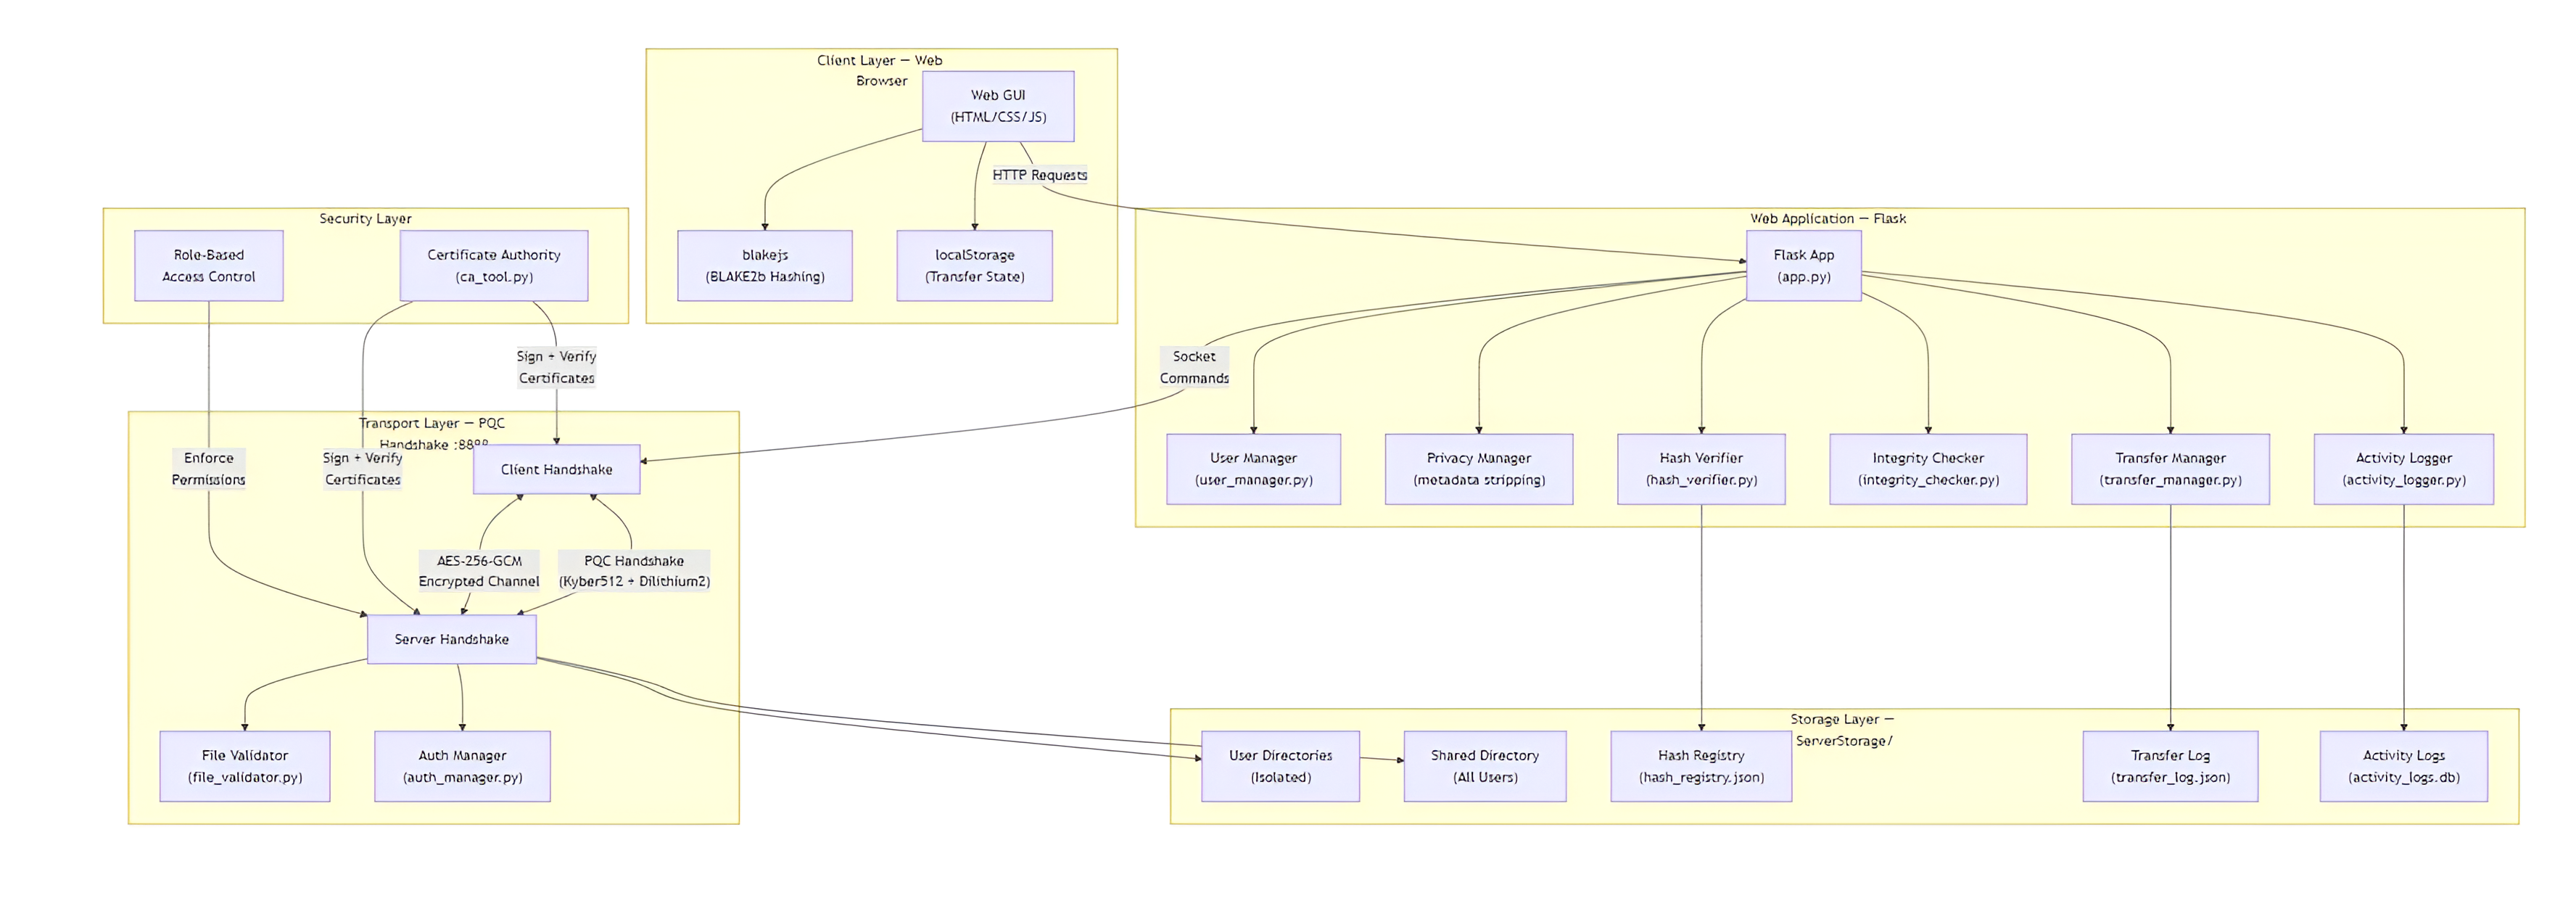
\includegraphics[width=\textwidth]{Figures/System_Architecture.png}
    \caption{Q-SFTP System Architecture — Four-Tier Modular Design}
    \label{fig:arch_diagram}
\end{figure}

\subsection{PQC Handshake Protocol Flow}

Figure~\ref{fig:pqc_diagram} illustrates the four-phase post-quantum handshake protocol: Hello Exchange, Kyber512 Key Encapsulation, Mutual Authentication via Dilithium2 transcript signing, and Secure Channel Establishment with HKDF-derived session keys.

\begin{figure}[H]
    \centering
    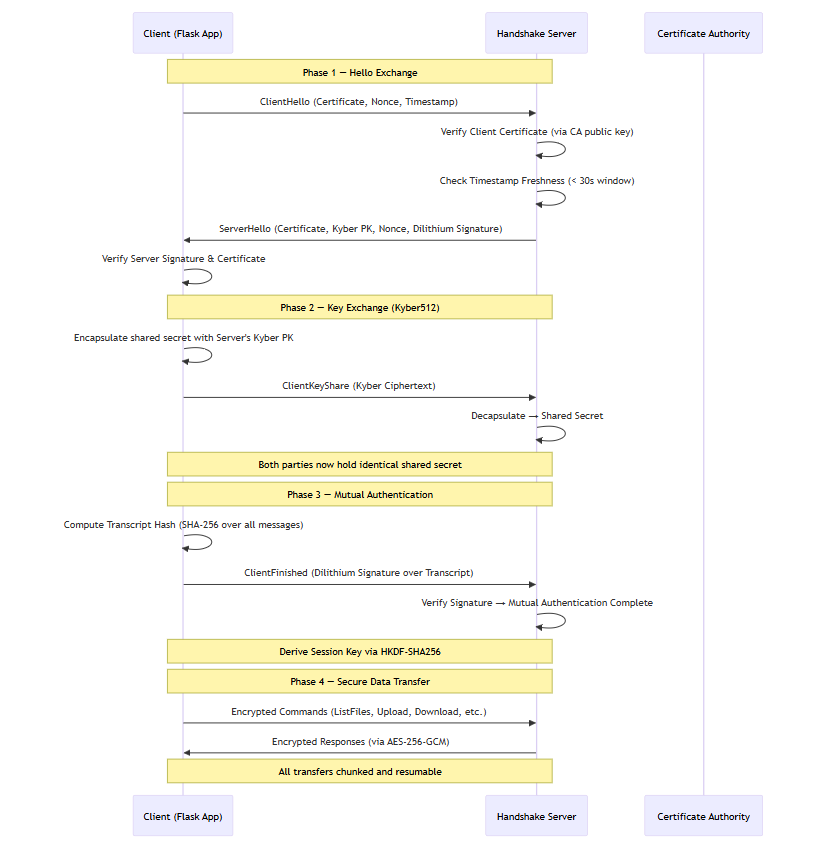
\includegraphics[width=\textwidth]{Figures/PQC_Handshake.png}
    \caption{PQC Handshake Protocol — Four-Phase Mutual Authentication}
    \label{fig:pqc_diagram}
\end{figure}

\subsection{Authentication and Session Flow}

Figure~\ref{fig:auth_flow} details the end-to-end authentication and session management flow, from user login through certificate-based PQC handshake to encrypted session establishment and subsequent file operations.

\begin{figure}[H]
    \centering
    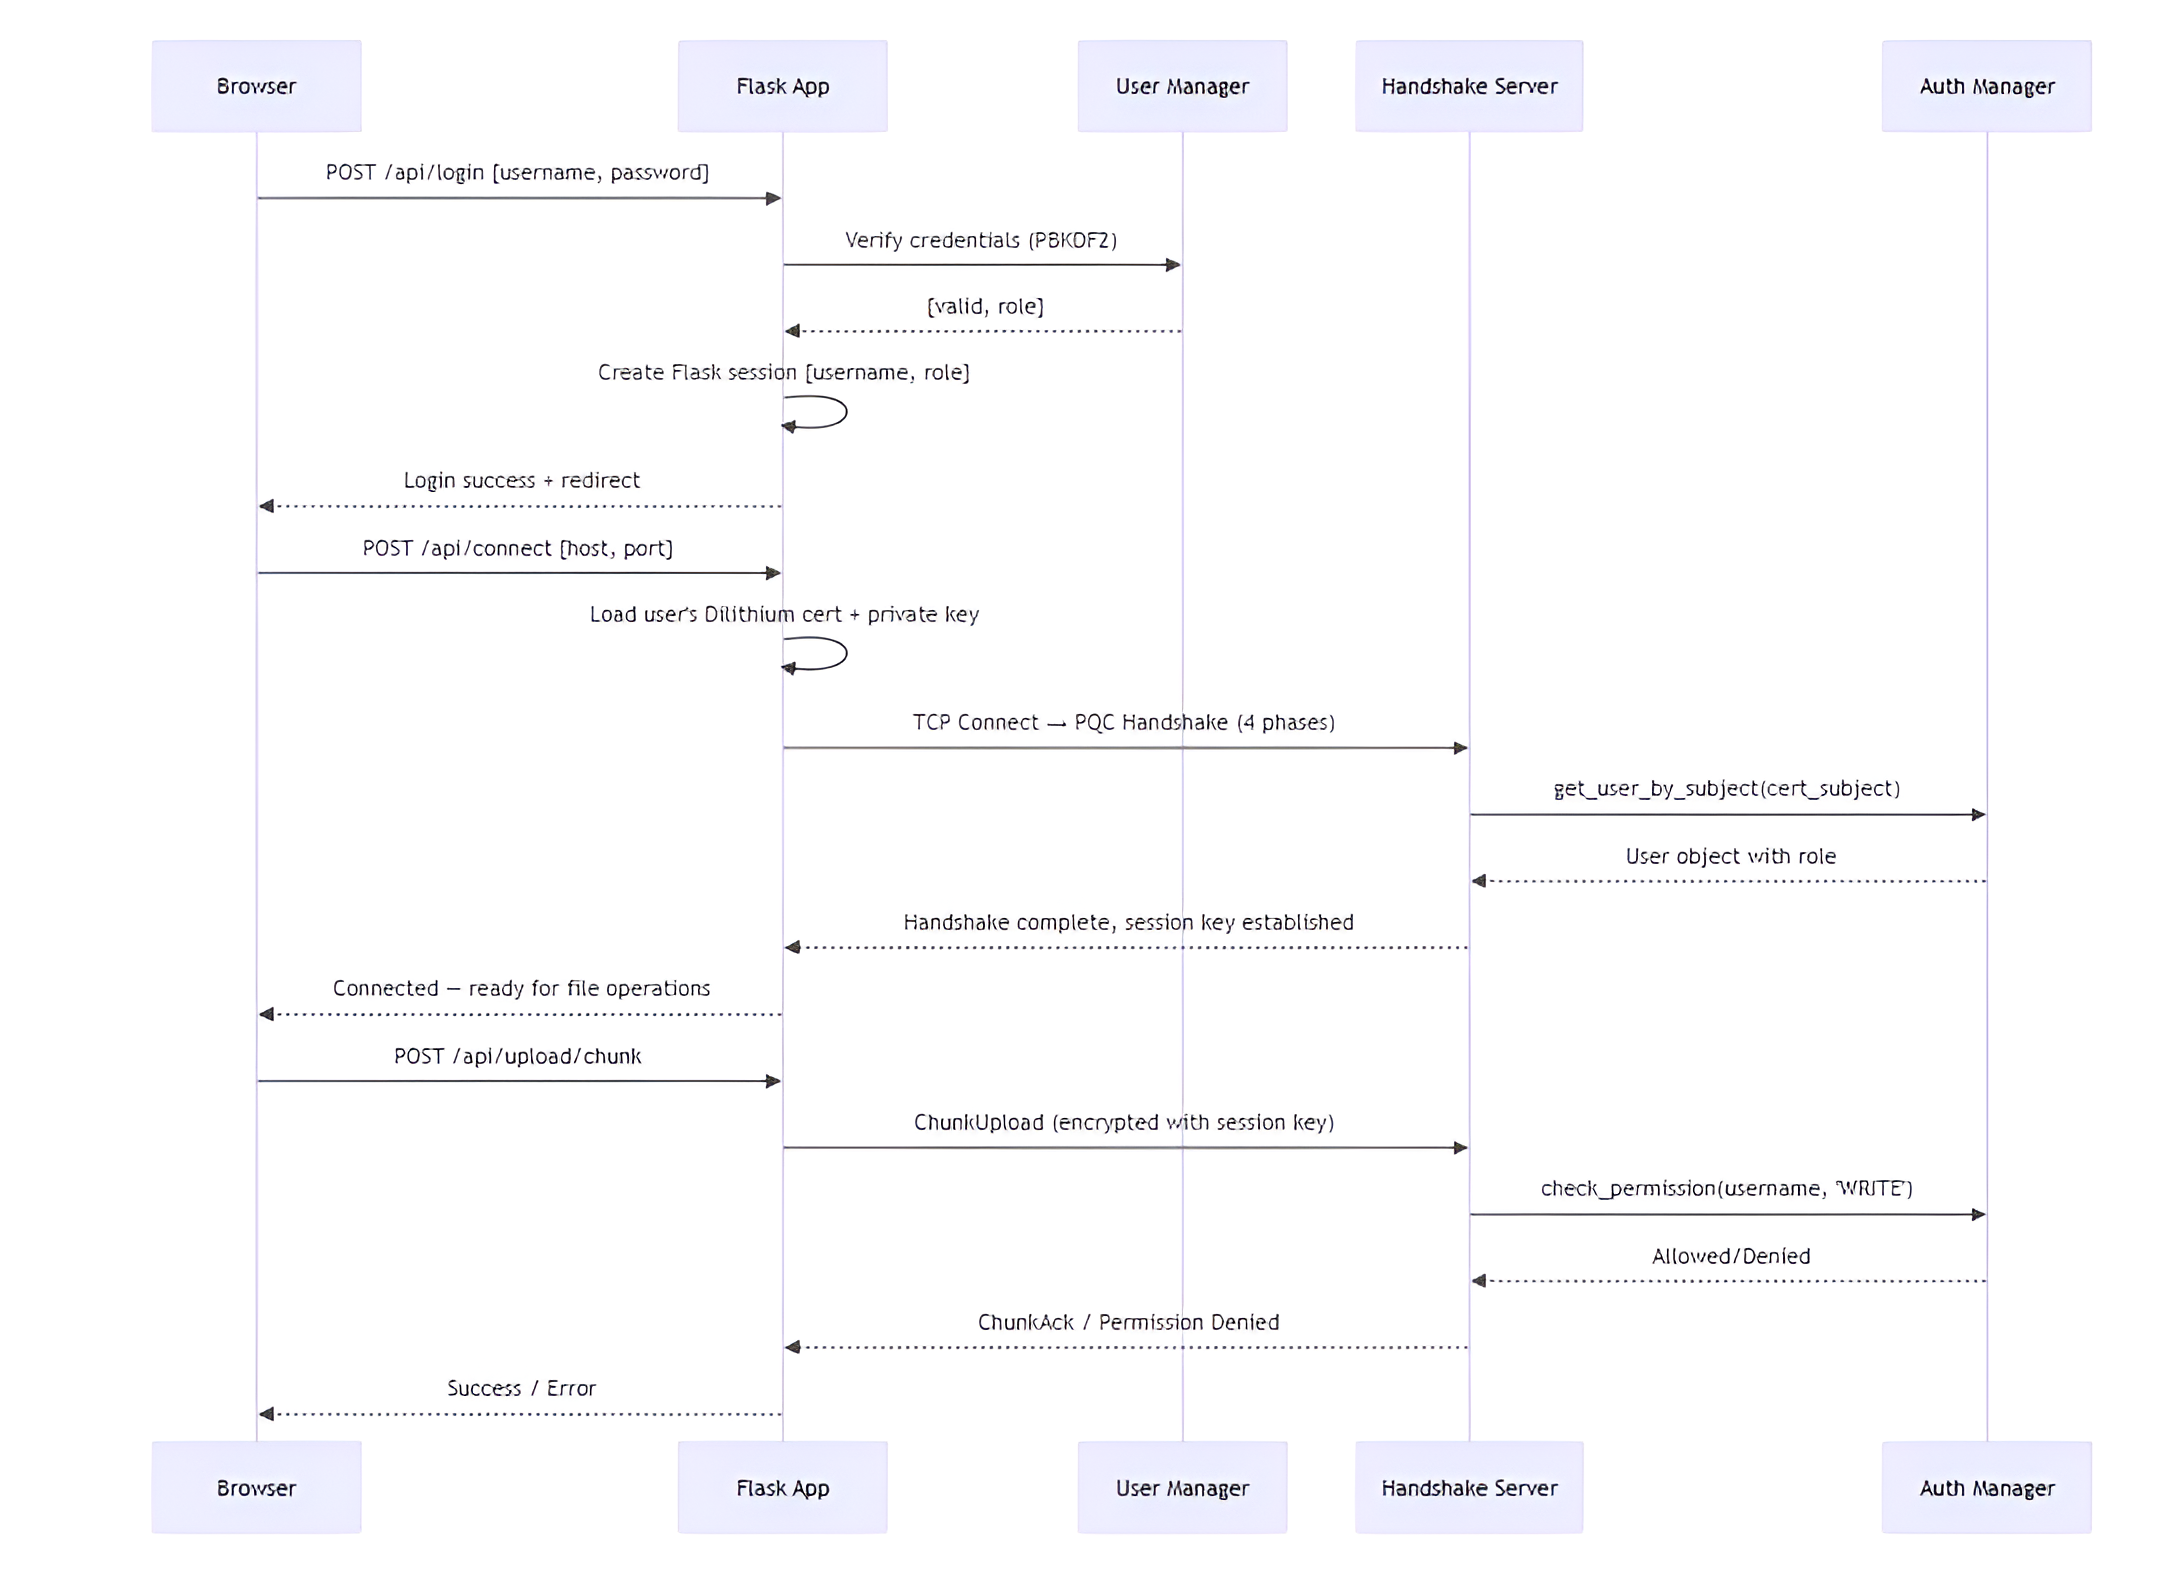
\includegraphics[width=\textwidth]{Figures/Authentication and Session Flow.png}
    \caption{Authentication \& Session Flow — Login to Encrypted File Operations}
    \label{fig:auth_flow}
\end{figure}

\subsection{Role-Based Access Control (RBAC)}

Figure~\ref{fig:rbac_diagram} visualizes the three-tier RBAC model with directory isolation, showing how Administrator, Standard, and Guest roles map to permitted operations and storage boundaries.

\begin{figure}[H]
    \centering
    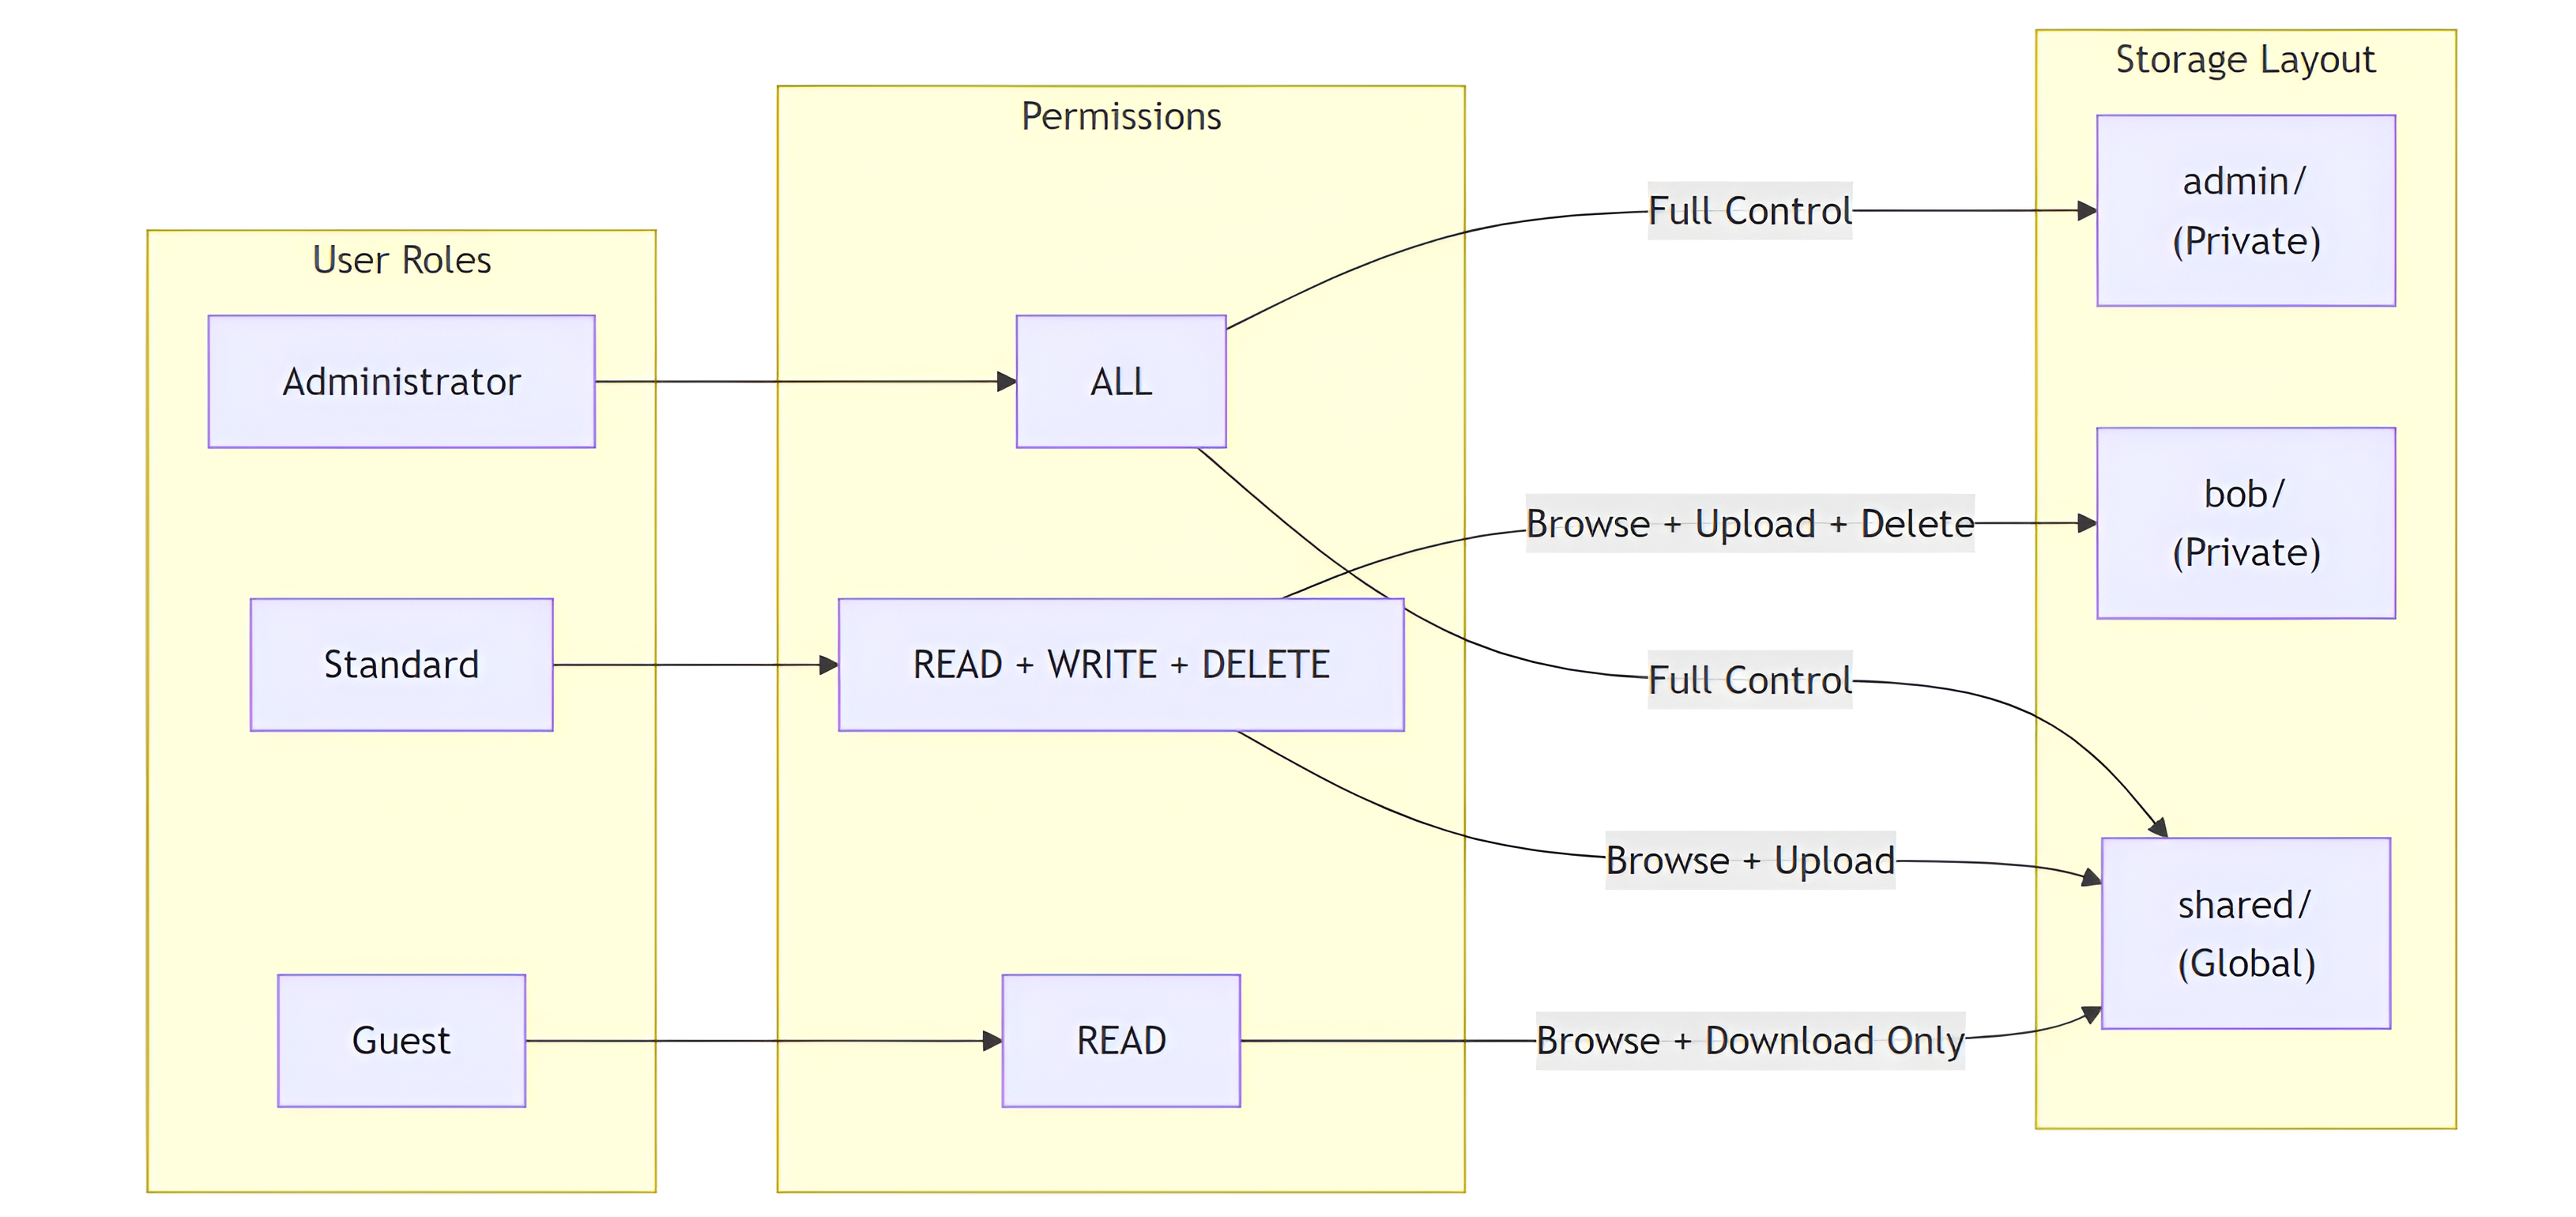
\includegraphics[width=\textwidth]{Figures/RBAC.png}
    \caption{Role-Based Access Control — Permission Model and Directory Isolation}
    \label{fig:rbac_diagram}
\end{figure}

\subsection{Resumable File Transfer Protocol}

Figure~\ref{fig:resume_diagram} depicts the chunked resumable transfer protocol, illustrating chunk processing, state persistence (client-side localStorage and server-side JSON log), and the resume-from-offset mechanism.

\begin{figure}[H]
    \centering
    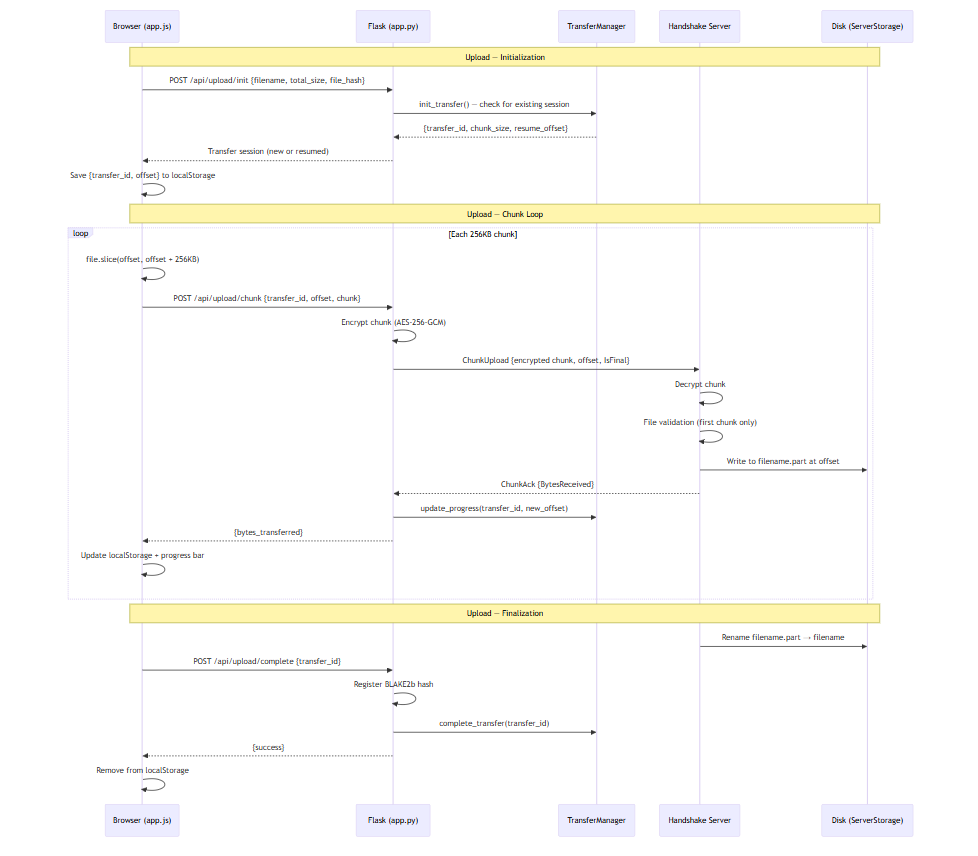
\includegraphics[width=\textwidth]{Figures/Resumable_File_Transfers.png}
    \caption{Resumable File Transfers — Chunked Protocol with State Persistence}
    \label{fig:resume_diagram}
\end{figure}

\section{Testing and Validation}

Testing was been performed to ensure that every module operates securely and efficiently:
\begin{itemize}
\item \textbf{Unit Testing:} Validates individual cryptographic operations (Kyber encapsulation/decapsulation, Dilithium signing/verification, BLAKE2b hashing).
\item \textbf{Integration Testing:} Validates the complete handshake flow between CA, server, and client modules, including certificate generation, mutual authentication, and session key derivation.
\item \textbf{Performance Testing:} Measures handshake latency, file transfer throughput, and chunk processing overhead.
\item \textbf{Security Validation:} Verifies resistance to replay attacks, certificate forgery, man-in-the-middle attacks, and file tampering.
\item \textbf{Hash Phase Testing:} A four-phase testing suite validates the hash infrastructure across registration, verification, tamper detection, and bulk operations.
\end{itemize}

For additional context, refer to Chapter~\ref{chap.2} for the background and Chapter~\ref{chap.3} for related work supporting the design rationale.
